
\section{Experiments}

In order to assess the improvement of our Deep Parameter Tuning approach, we compared our approach with the Shallow Parameter Tuning approach and posed the following research questions: 
 

\begin{description}
 \item[RQ1] {\bf How much improvement on performance can be obtained by Shallow Parameter Turning, compared with the original, using random search and NSGAII? }
\end{description}

We asked RQ1 to provide us a baseline result against which we compare the results from Deep Parameter Tuning. To mimic a traditional Shallow Parameter Tuning approach, we used the same NSGAII algorithm introduced in Section \ref{sec_nsgaii} to search for the optimal values for the default explicit parameters in \emph{dlmalloc}. To answer this question, we compared the performance of the optimised configuration found by NSGA II with the default \emph{dlmalloc} configuration and the best configurations found by random search with the same computation budget.  

\begin{description}
\item[RQ2] {\bf How much more improvement can be achieved by Deep Parameter Tuning compared with Shallow Parameter Tuning? }
\end{description}

We ask the RQ2 to see how useful our approach is at finding better configurations for the given non-functional properties. Our Deep Parameter Tuning approach uses Mutation Operators to identify the most sensitive parts of the program, followed by applying NSGAII to optimise both explicit and implicit parameters for \emph{dlmalloc}. %Of course, should it turn out that the Shallow Parameter Tuning approach can find as good configuration as that by our approach, then our approach would not be needed. 

\begin{description}
\item[RQ3] {\bf Do we see evidence that our Deep Parameter Tuning approach can expose implicit parameters which are meaningful to human developers? }
\end{description} 

Should it turn out that the Deep Parameter Tuning approach performs well, achieving much improvement than the Shallow Parameter Tuning approach, then we have evidence to suggest that the mutation based sensitivity analyse used in our approach is able to locate the inner expressions or variables which are sensitive to the given non-functional properties. However, do these inner expressions or variables also make sense to software developer? To answer this research question, we manually investigate the exposed variable and try to learn why tuning these parameters can make \emph{dlmalloc} more efficient.  


\subsection{Dlmalloc}

Dynamic memory allocation is an essential activity in most of the applications. It happens when an application needs a piece of memory whose size cannot be determined until runtime. Most systems support some system calls that could dynamically assign some memory to an application. When an application asks for some dynamic memory from the operating system, the simplest way is to give the exact size of memory it requests through these system calls, and to retrieve that memory back as soon as the application frees it. However, these allocation and deallocation system calls are usually much slower than other operations. So frequently allocating memory directly from the system is impractical for most of the applications. 

Memory allocators have risen to solve this problem using different allocation strategies. Usually applications communicate with the operating system in terms of memory only through their memory allocators. The idea of these allocators is trying to hold and manage some extra memory applied from the system and use them to serve latter memory request from the application as effiecently as possible. On the other hand, when a piece of memory is freed by the application, before released to the system it is handled by memory allocators in case there is a memory request in the same size in the near future. So it works like a memory buffer between an application and the system. Different ways of memory management significantly influence the performance of an application in terms of both memory and time.

Many memory allocation strategies and managers have been proposed and studied by many researchers. Among them, Doug Lea's malloc (\emph{dlmalloc}) \cite{lea1996memory} is ``among the fastest, most space-conserving, tunable, and portable general purpose allocators''. A study of Berger et al\cite{Berger:2002:RCM:583854.582421} shows that many other custom memory allocators don't perform significantly better than \emph{dlmalloc}, sometimes even worse. So in this paper, we choose \emph{dlmalloc} as our starting point and optimize its configuration to each of the subject applications.

%\begin{figure}[htbp]
%\centering
%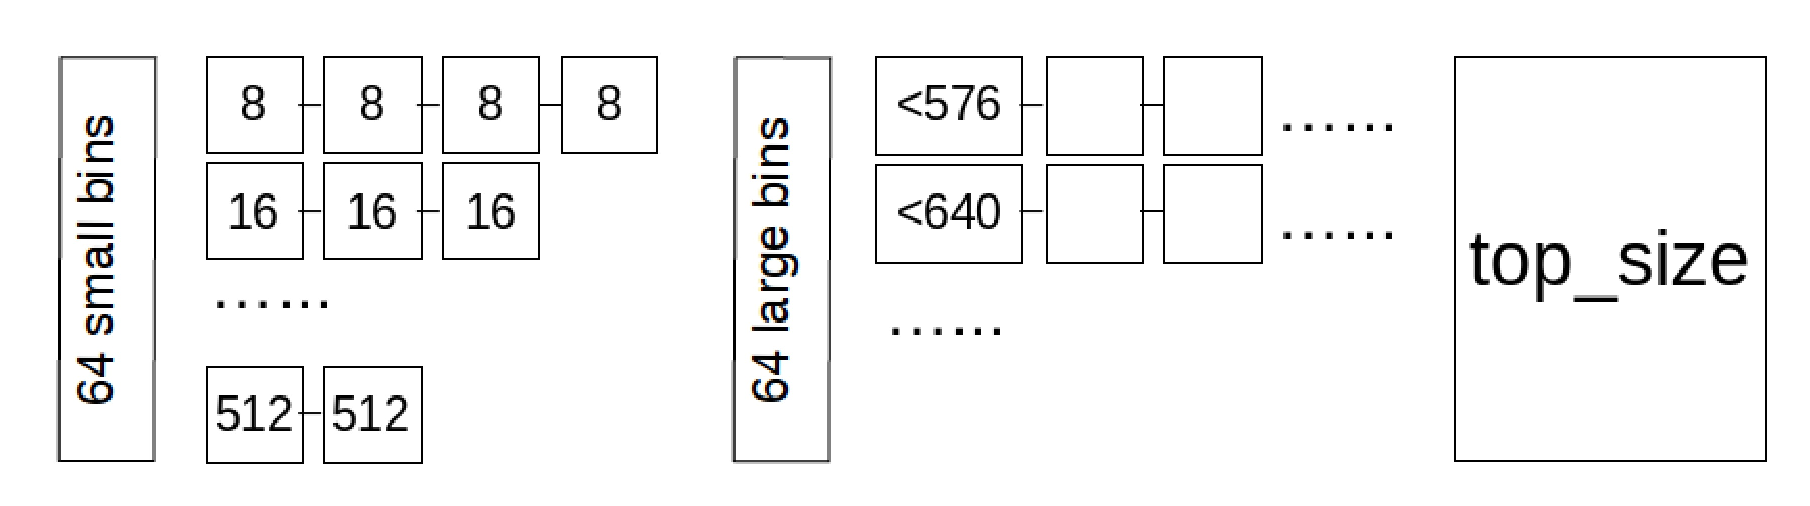
\includegraphics[width=3.2in]{fig7}
%\caption{structure of \emph{dlmalloc}}\label{fig_7}
%\end{figure}

\emph{Dlmalloc} is a general purpose memory allocator designed for c programs. In most of the cases, it is used with its default configuration while it provide the possibility to re-configure the parameters. We call these configurable parameters provided by the original author Shallow Parameters, from which we choose 9 Shallow Parameters that are more likely to influence the time and memory performance based on our understanding.

For example, \textbf{MALLOC\_ALIGNMENT} represents a multiple of how many bytes all request sizes should be rounded up to. It is an essential parameter since many other parameters are derived from it to avoid incompatibility. Smaller MALLOC\_ALIGNMENT tends to save memory but may not be compatible with all applications. Table \ref{tab_dlmalloc_parameters} lists all 9 Shallow Parameters and brief description for them.
%It keeps two set of segregated lists managing small and large size available chunks respectively. Each of the segregated lists is called a bin and there are 64 small bins and 64 large bins in \emph{dlmalloc} (Figure \ref{fig_7}). For small bins, each one contains chunks in the exact same size, in which way insertion to or deletion from the list is very quick. For large bins, each bin is associated with a range of sizes and any free chunks within that range are stored in the corresponding bin in the ascending order. So managing large bins is more costly than small bins but fortunately large bins are less frequent than small bins. Apart from these bins, \emph{dlmalloc} also keeps a top chunk, which is always at the end of the heap so that it can be extended or trimmed without affecting other memory chunks. 

%The top chunk is used only when there is no available chunk in any bins that meets the memory request. If the request size is too large to be satisfied from the top chunk and bigger than a pre-defined threshold, \emph{dlmalloc} uses an \emph{mmap}-like system call to allocate this size of memory from the operating system directly. Or it tries to extend the top chunk using \emph{sbrk}-like system call, so that the extended top chunk is big enough to cover the request.
%When a chunk is freed by the application, it is put back to one of the bins according to its size, after which \emph{dlmalloc} occasionally coalesces contiguous free chunks to create bigger chunks. If the top chunk is enlarged by combining free chunks next to it, it could be trimmed if it is too large for the need of the application if the freed chunk was mapped directly from the system, it is released to the system immediately. 

% Intruduce the 9 parameters defined in Dlmalloc (1 paragraph)
% draw a table with "para name, type, range, default, comment"
\begin{table*}[htbp]
\centering
\caption{Selective \emph{dlmalloc} parameters}
\label{tab_dlmalloc_parameters}
\resizebox{0.9\textwidth}{!}{
\begin{tabular}{c|c|c|c|c}
\hline
Name & Default & Range & Type & Description\\
\hline
MALLOC\_ALIGNMENT & $2*sizeof(void*)$ & $(1~16)*sizeof(void*)$ & $2^n*sizeof(void*)$ & Alignment unit\\
\hline
FOOTERS & \emph{false} & \emph{true} or \emph{false} & boolean & Additional information of each chunk\\
\hline
INSECURE & \emph{false} & \emph{true} or \emph{false} & boolean & Secure check\\
\hline
NO\_SEGMENT\_TRAVERSAL & \emph{false} & \emph{true} or \emph{false} & boolean & Traversal of chunks before coalescing\\
\hline
MORECORE\_CONTIGUOUS & \emph{true} & \emph{true} or \emph{false} & boolean & Contiguous heap extension support\\
\hline
DEFAULT\_GRANULARITY & 0 & 4KB - 512KB & $2^n$KB or 0 & Unit of heap extension\\
\hline
DEFAULT\_TRIM\_THRESHOLD & 2048KB & 64KB - 16MB & $2^n$KB & Threshold of trimming\\
\hline
DEFAULT\_MMAP\_THRESHOLD & 256KB & 16KB - 2MB & integer & Threshold of direct memory mapping\\
\hline
MAX\_RELEASE\_CHECK\_RATE & 4095 & 1000 - 10000 & integer & Frequency of coalescing\\
\hline
\end{tabular}}
\end{table*}

%\subsection{Dlmalloc tunable parameters}
%\label{sec_dlmalloc_tunable_parameters}
%As a general-purpose allocator, \emph{dlmalloc} provides several tunable parameters to programmers to adjust at compilation. More specifically, these parameters are defined as macros in the source code, but can be modified via compilers (we achieve that through \emph{gcc}'s ``-D'' flag). We call them Shallow Parameters. In this article, we choose some of these parameters that are more likely to influence the allocator's behavior in terms of memory/time consumption, as our ``victims''. 
%
%One of the core parapemter macros in \emph{dlmalloc}  is \textbf{MALLOC\_ALIGNMENT}. It represents a a multiple of how many bytes all request sizes should be rounded up to. Many of other macros in \emph{dlmalloc} rely on this alignment to avoid any incompatibility. Its default value is $2*sizeof(void*)$ where $sizeof(void*)$ varies across different systems. Normally smaller MALLOC\_ALIGNMENT tends to save more memory but could also cause incompatibility with some applications. 
%
%For the sake of brevity, only two of them are detailed as examples. \textbf{MALLOC\_ALIGNMENT} is one of the most basic macros in \emph{dlmalloc}, representing a multiple of how many bytes all request sizes should be rounded up to. Most of other macros in \emph{dlmalloc} rely on this alignment to avoid any incompatibility. Its default value is $2*sizeof(void*)$ where $sizeof(void*)$ varies across different systems. Normally smaller MALLOC\_ALIGNMENT tends to save more memory but could also cause incompatibility with some applications. 
%
%\textbf{DEFAULT\_MMAP\_THRESHOLD} is the size bigger than which a request that can not be served via existing free chunks, is allocated through \emph{mmap}-like system call. These \emph{mmap}ed chunks can not be consolidated or reuse by other request, but unlike regular chunks, they never get trapped by other ocuppied chunks, meaning they can be directly released to the system as soon as the application frees it. Bigger DEFAULT\_MMAP\_THRESHOLD tends to cause more memory consumption but save allocation time. The default, 256KB, is ``an empirically derived value that works well in most systems''. A list of the parameters we target in this article is given in Table \ref{tab_dlmalloc_parameters}. More detailed description of these parameters can be found in the comments of \emph{dlmalloc} source code.


\subsection{Experiment Setup}


\begin{table}[htbp]
\centering
\caption{Subject applications}
\label{tab_sub_app}
\resizebox{0.5\textwidth}{!}{
\begin{tabular}{|c|r|r|l|}
\hline
Name & Loc & No. of tests & Type \\
\hline
espresso & 13256 & 19 & Digital electronic gate circuits simplification\\
\hline
gawk & 45241 & 334 & String processing\\
\hline
flex & 9597 & 62 & Fast lexical analyzer\\
\hline
sed & 5720 & 362 & Special file editor\\
\hline
\end{tabular}}
\end{table}

For our evaluation, we selected four real world applications: \emph{espresso}, \emph{gawk}, \emph{flex} and \emph{sed}. \emph{Espresso} is a fast application for simplying complex digital electronic gate circuits. We use the source code and test cases from the \emph{DieHard} project \cite{Berger:2006:DPM:1133255.1134000}. \emph{Gawk} is the GNU \emph{awk} implementation for strings processing. We collect this application as well as its testsuite from the GNU archives. \emph{flex} is a tool for generating scanners, programs which recognizes lexical patterns in text, and \emph{sed} is a special editor that automatically modifies files given a set of changing rules. We obtain these last two programs and corresponding testsuite from the SIR repository \cite{SIR2005}. A more detailed description for these subject programs is list in Table \ref{tab_sub_app}.
% and \emph{cfrac} is a factorization application for big integers. We obtain these two applications from the benchmarks of the \emph{DieHard} project \cite{Berger:2006:DPM:1133255.1134000}. \emph{Space} is a well known real world application in astronautics. We obtain this program from the SIR repository \cite{SIR2005}. \emph{Gawk} is the GNU \emph{awk} implementation for strings processing. We collect this application from the GNU archives.
%
%Although tuning parameter of malloc is less likely to change the behaviour of our subjects under optimise directly, some combination of unusual parameters' values could also crash a subject system. To make sure the configuration generated by our approach always prodcue the same functional results as the default configuration, we use the number of passed tests as an addtional hard constraints. We used the tests from the \emph{DieHard} project for \emph{Espresso} and \emph{cfrac} and the tests from SIR for \emph{Space}. These tests are designed by programmer and achieve high branche coverage. For \emph{gawk}, because the existing test cases are too small to precisely capture the running time, we manually generate a test suite which achieves ** branch coverage.


\subsection{Experiment Procedures}

We first used the Shallow Parameters only and applied NSGAII algorithm with a population of 50 for 300 generations to search for the optimal values. A random search was also applied with the same computation budget in optimising the Shallow Parameters. Then we applied selective Mutation Operators to gather the sensitivity information and expose 9 Deep Parameters (the same number with the Shallow Parameters) for each subject program separately, as described in section \ref{sec_deep_parameter_optimisation}. Combining Shallow and Deep Parameters, we again applied NSGAII to search for the optimal values for each of the subject programs. All experiments were repeated for 30 runs to have a statistics conclusion.

All experiments were carried out on virtual machines with a double-core CPU and \# GB memory runing **64-bit Ubuntu 13.10 on Azure cloud platform. We used \emph{dlmalloc} version 2.8.6, which was compiled with gcc 4.8.1 with -O3 option. In order to capture the execution time and memory consuming precisly, we developed our own performance tool to measure the CPU time and the high-water-mark vitural memory consumption (see Section \ref{sec_nsgaii}). The tool is publicly available at **www.fan.put.a.link.later.
%(**describe how we apply our approach on the dlmalloc case study, including separately finding best locations to expose with respect to each subject application)
%(**mention we use NSGA II to optimize both Deep and Shallow parameters after we expose Deep Parameters from each subject. reference the section describing Shallow Parameter and NSGA II)
